\documentclass[11pt,a4paper]{article}
\usepackage[hyperref]{acl2020}
\usepackage{times}
\usepackage{latexsym}
\renewcommand{\UrlFont}{\ttfamily\small}
\usepackage{microtype}
\newcommand\BibTeX{B\textsc{ib}\TeX}
\usepackage{xcolor}
\usepackage{graphicx}
\usepackage{placeins}

\aclfinalcopy % Uncomment this line for the final submission
\title{Etymological Embeddings for Contextless Definition Modeling}
\author{Noah Gardner \\
  Kennesaw State University \\
  College of Computing and Software Engineering \\
  \texttt{ngardn10@students.kennesaw.edu} \\}

\begin{document}
\maketitle
\begin{abstract}
  Definition modeling is the problem of estimating the probability of an output
  definition given an input word embedding. There exist some methods of creating
  word embeddings concatenated that take the input word concatenated with the
  context of the word. However, the context is not always available.
  Additionally, progress has been made in research for \textit{etymology
    modeling} where the etymology of a word can be estimated from the input word
  embedding. In this paper, we propose a definition modeling method that uses
  etymological information.
\end{abstract}

\section{Introduction}
Word embeddings are vector representations of words that allow us to use words
as inputs to machine learning models for natural language processing tasks
\cite{mikolov_efficient_2013}. There are many word embedding methods that
achieve state-of-the-art performance on NLP problems, such as sentiment
analysis. Addtionally, contextualized word embeddings have been shown to improve
performance with models such as ELMo and BERT \cite{peters_deep_2018,
  devlin_bert_2019}.

Dictionary definitions can yield value for sentiment aware models, however,
crowdsourced annoations are costly. The task of definition modeling was proposed
to address this problem. The goal of definition modeling is to estimate the
probability of an output definition given an input word embedding
\cite{noraset_definition_2016}.

Wiktionary\footnote{wiktionary.org} is a free online dictionary that provides
details about many words, including definitions, etymologies, pronounciation,
and examples. Some research has used the large data dumped from Wikitionary to
support NLP research such as etymology modeling and word sense disambiguation
\cite{wu_computational_2020}.

The etymology of a word is a tree structure that describes the word's origin.
Although contextualized embeddings show improvement in NLP tasks, the context of
a word is not always available. With advances in etymology modeling, if we know
the source language of a word, we can predict the etymology of the word. Using
this observation, we propose a word embedding with etymological information for
the task of definition modeling. This work intends to show improvement for
contextless definition modeling, although it may be used in conjuction with a
contextualized embedding for even better performance.

\section{Related Work}

Definition modeling was intially described by \citet{noraset_definition_2016}.
Their research is based on a recurrent neural network language model
\cite{mikolov_recurrent_2010} with a modified recurrent unit. They use the word
to be defined placed at the beginning of the definition so the model will see
the word only on the first step.

\citet{chang_what_2019} explore contextualized embedding for definition
modeling. They reformulate the problem of definition modeling from text
generation to text classification. Their results show state-of-the-art
performance on the task of definition modeling.

\citet{washio_bridging_2019} proposed a method for context-based definition
modeling that considers the semantic relations between both the word to be
defined and the words in the definition. They apply semantic information to both
the definition encoder and decoder.

\citet{barba_exemplification_2021} introduce exemplification modeling, an
adjacent problem to definition modeling that uses a definition embedding to
generate possible example sentences. They use a sequence-to-sequence based
approach and show near human-level annotation performance. Their problem is
similar in that they use the definition as context to create example sentences.

\section{Overview}

This section will provide an overview of the different works required to solve
the problem of definition modeling with embeddings.

\subsection{Raw Dataset}
In this subsection, we investigate the parsed wikitionary dump from
\citet{wu_computational_2020} and discuss the relevant aspects of the dataset.

\subsubsection{Definition}

\begin{table}[h]
  \centering
  \begin{tabular}{|l|l|}
    \hline
    \textbf{Word} & \textbf{Definition}             \\
    \hline\hline
    free          & $(lb|en|social)$ Unconstrained. \\
    free          & Not imprisoned or enslaved.     \\
    free          & Generous; liberal.              \\
    \hline
  \end{tabular}
  \caption{Parsed wikitionary example definitions for the english word
    \textit{free}.}
  \label{tab:wiktionary_definitions}
\end{table}

The definition dataset includes information on the source language, the word to
be defined, the part of speech, and the defintion of the word. The definition of
a word can also contain a specific context in which the definition is used.
Figure \ref{tab:wiktionary_definitions} shows some example definitions from the
dataset for the word \textit{free}.

\subsubsection{Etymology}

Similar to the definition dataset, the etymology dataset includes information on
the source language, the word to be analyzed, and the etymology of the word. The
etymology is a tree structure that describes the word's origin, including roots
from other languages. Figure \ref{fig:wiktionary_etymology} shows an example
etymology from the dataset for the word \textit{free}.

\begin{figure}[h]
  \color{blue}free \color{black}[\color{green}(eng|free)\color{blue}(root)\color{red}(eng|ine-pro|*preyH-)\color{black}]
  \caption{Parsed wikitionary example etymology for the english word
    \textit{free}.}
  \label{fig:wiktionary_etymology}
\end{figure}

\subsection{Embeddings}

In this subsection, we will investigate how we can create definition embeddings
for definition modeling.

\subsubsection{Universal Sentence Encoding}

In order to create defintions, we need to obtain the embedding of the definition
we wish to predict. We also must obtain embeddings of the input word and
context. By using a pre-trained universal sentence encoder, we can obtain
embeddings for both the inputs and the expected outputs.

\subsubsection{Defintion Embedding Prediction}
Once we have the input embeddings and expected output embeddings, we can train a
model to predict the output embedding. In general, the problem of definition
modelling is a text generation problem. We may also solve the problem as a
classification task. That is, predict the closest definition in the dataset to
the predicted embedding using a distance metric such as cosine similarity, the
proposed approach of \citet{chang_what_2019}.

In their experiments, after creating a contextualized embedding as well as a
word embedding, both are used as inputs to a convolutional neural network. The
resulting model is able to predict a definition embeddinggs for the given input.
This approach allows them to avoid some of the pitfalls of text generation, such
as problems associated with greedy search and generating grammatically correct
sentences.

With the predicted definition embedding, we compare the predicted embedding to
definition embeddings in the dataset. Using an approach similar to the
$k$-nearest neighbor algorithm, we may find $k$ definitions that are most
similar to the predicted embedding.

\section{Methodology}

\subsection{Dataset}

From the definition and etymology datasets, we use only the words with the
english source language. For the defintions, we remove self-referential
defintions and utilize a maximum of three definitions per word. Although the
context-based definitions may provide some benefit for a context-based model, we
remove the context from the definitions. Additionally, the definition of some
words are completely context (such as alternate spellings) and are also removed.
Fue to background limitations, rather than use the entire etymology tree to
generate our etymological embeddings, we use only the first etymology for each
word if there exist multiple. Finally, we ignore words tagged with
\textit{proper noun}. Dataset statistics are shown in Figure
\ref{tab:dataset_stats} after the described steps are applied.

\begin{table}[h]
  \centering
  \begin{tabular}{|l|l|}
    \hline
    \textbf{Type}                & \textbf{Amount} \\
    \hline\hline
    Unique Words                 & \textbf{320855} \\
    Average Definitions Per Word & \textbf{1.288}  \\
    Etymology (Average Length)   & \textbf{41.725} \\
    Definition (Average Length)  & \textbf{51.711} \\
    \hline
  \end{tabular}
  \caption{Dataset statistics for the combined datasets.}
  \label{tab:dataset_stats}
\end{table}

\subsection{Models}

A simple sketch of the proposed approach can be found in Figure
\ref{fig:proposed_approach}.

\subsubsection{Encoder Model}
BERT \cite{peters_deep_2018} is a commonly used encoder for the task of creating
sentence embeddings due to it's ability to contextualize information with both
forward and backward passes. However, we are working with limited resources and
must choose a model with fewer parameters. Therefore, we have chosen the DeCLUTR
model for unsupervised textual representation \cite{john_decluter_2020}. Aside
from being readily accessible in the huggingface library, it is a useful model
due to its unsupervised nature.

\subsubsection{Prediction Model}
As described in the Overview section, we are using a classification-based
approach for definition modelling. After our word, definition, and etymology
embeddings are created, we use a simple dense neural network with 3 hidden
layers to predict the closest definition to the predicted embedding. In order to
train the model, we select a set of unique words from the dataset and use them
as the input words. The leftover set of words is used for testing. In other
words, any word that appears in the training set is does not appear in the
testing set.

\subsubsection{Definition Selection}
Once we have predicted a definition embedding, we use a distance metric to find
the closest 3 definitions to the predicted embedding. We use cosine similarity
as our distance metric and use an approach similar to the $k$-nearest neighbor
algorithm. Unfortunately, most of the metrics used in definition modelling
cannot be applied to this approach as the metrics expect a generated embedding
rather than the complete defintion from the dataset.

\begin{figure}
  \centering
  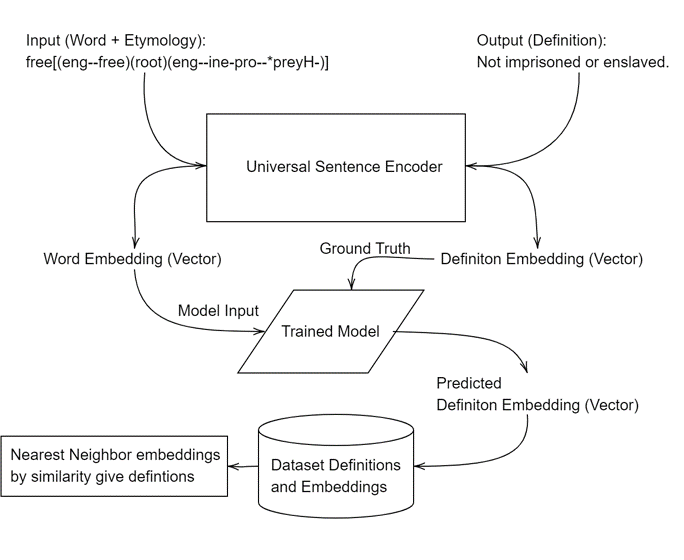
\includegraphics[width=0.48\textwidth]{assets/proposed_approach.png}
  \caption{Overview of the proposed approach for definition modelling with a
    sample input.}
  \label{fig:proposed_approach}
\end{figure}

\section{Experimental Results}
Due to the lack of quantitative metrics for a classification-based definition
modelling approach, we simply show some of the best cosine similarity scores for
predicted embeddings, shown in Figure \ref{fig:best_words}. We also show some
generated definitions in Figures \ref{fig:generated_definition_1} and
\ref{fig:generated_definition_2}.

\begin{figure}
  \centering
  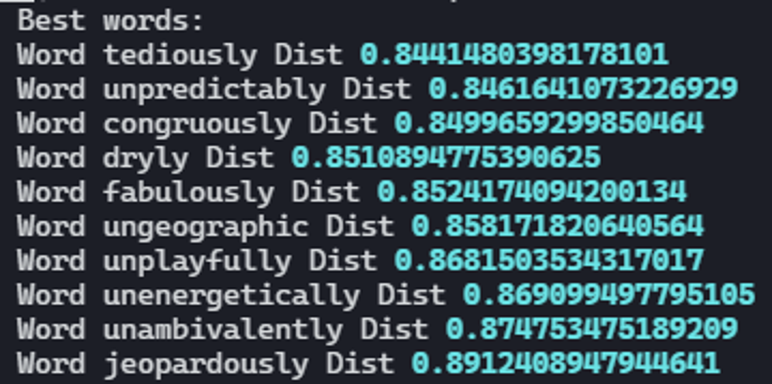
\includegraphics[width=0.48\textwidth]{assets/best_words.png}
  \caption{Best cosine similarity scores for the predicted embeddings.}
  \label{fig:best_words}
\end{figure}

\begin{figure}
  \centering
  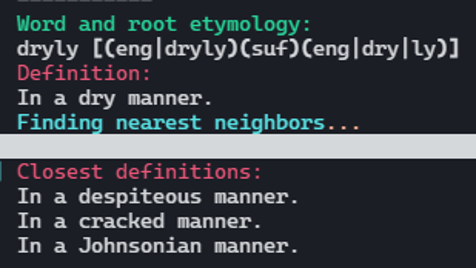
\includegraphics[width=0.48\textwidth]{assets/dryly_defs.png}
  \caption{Generated definitions for the word \textit{dryly}.}
  \label{fig:generated_definition_1}
\end{figure}

\begin{figure}
  \centering
  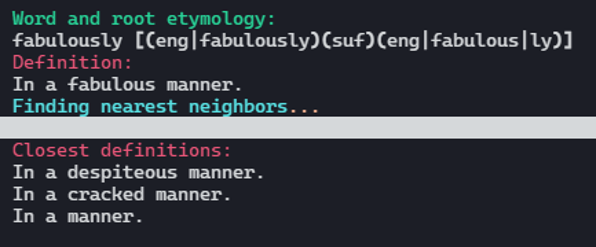
\includegraphics[width=0.48\textwidth]{assets/fabulously_defs.png}
  \caption{Generated definitions for the word \textit{fabulously}.}
  \label{fig:generated_definition_2}
\end{figure}

\FloatBarrier
\section{Conclusion}
In this paper, we provided a method of using etymological embeddings instead of
contextualized embeddings for the problem of definition modelling. However, the
problem of generating sentences from embeddings is a difficult topic.
Additionally, due to limited understanding of the author, we use a simplified
etymological tree rather than the entire structure. The experimental results
show that the model scores best on adverbs ending in \textit{ly}, and the best
defintions are all sentences of the form "\textit{In a $\_$ manner.}". This
shows either a problem with models used or our approach, as the model is stuck
in a local minima of definitions that are technically similar but not
necessarily correct to the expected definitions. Future work should address this
issue by testing strong models, using the entire etymology tree, and using a
more advanced approach to dataset setup. If these approaches can be tested, we
believe etymological embeddings have the ability to be as useful as context in
the task of definition modelling.

\section*{Acknowledgments}
This work was supported by computational resources provided by the Kennesaw
State University Department of Electrical and Computer Engineering.

\bibliography{report.bib}
\bibliographystyle{acl_natbib}
\end{document}
